\chapter{Resultados Preliminares}

\section{Mezuro: Prezento}

% TODO: falar sobre o Prezento, pois será a camada em que irei trabalhar

% TODO: atualizar versões citadas do RoR que o Mezuro utiliza

Como dito no capítulo anterior, o Prezento é a camada da interface web do
Mezuro. Desenvolvido em Ruby on Rails, atualmente utiliza as versões 2.2.3 do
Ruby e 4.2.4 do Rails. Versões estas que estão em constante mudança, pois os
autores têm como intuito usufruir o que há de mais recente das funcionalidades
dessa tecnologia. Esta será a principal camada trabalhada neste trabalho de
conclusão de curso, pois é
nela que há a interação com o usuário. Possivelmente será utilizado um botão que
possibilitará ao usuário ter acesso e interagir com a visualização gráfica do
resultado da análise estática na mesma página ou em outra. As Figuras
\ref{fig:exmplo_disposicao_botao_visualizacao_1} e
\ref{fig:exmplo_disposicao_botao_visualizacao_2} mostram possíveis localizações
para este botão.

% TODO: atualizar estas imagens e DESTACAR botôes

\begin{figure}[!htb]
	\centering
    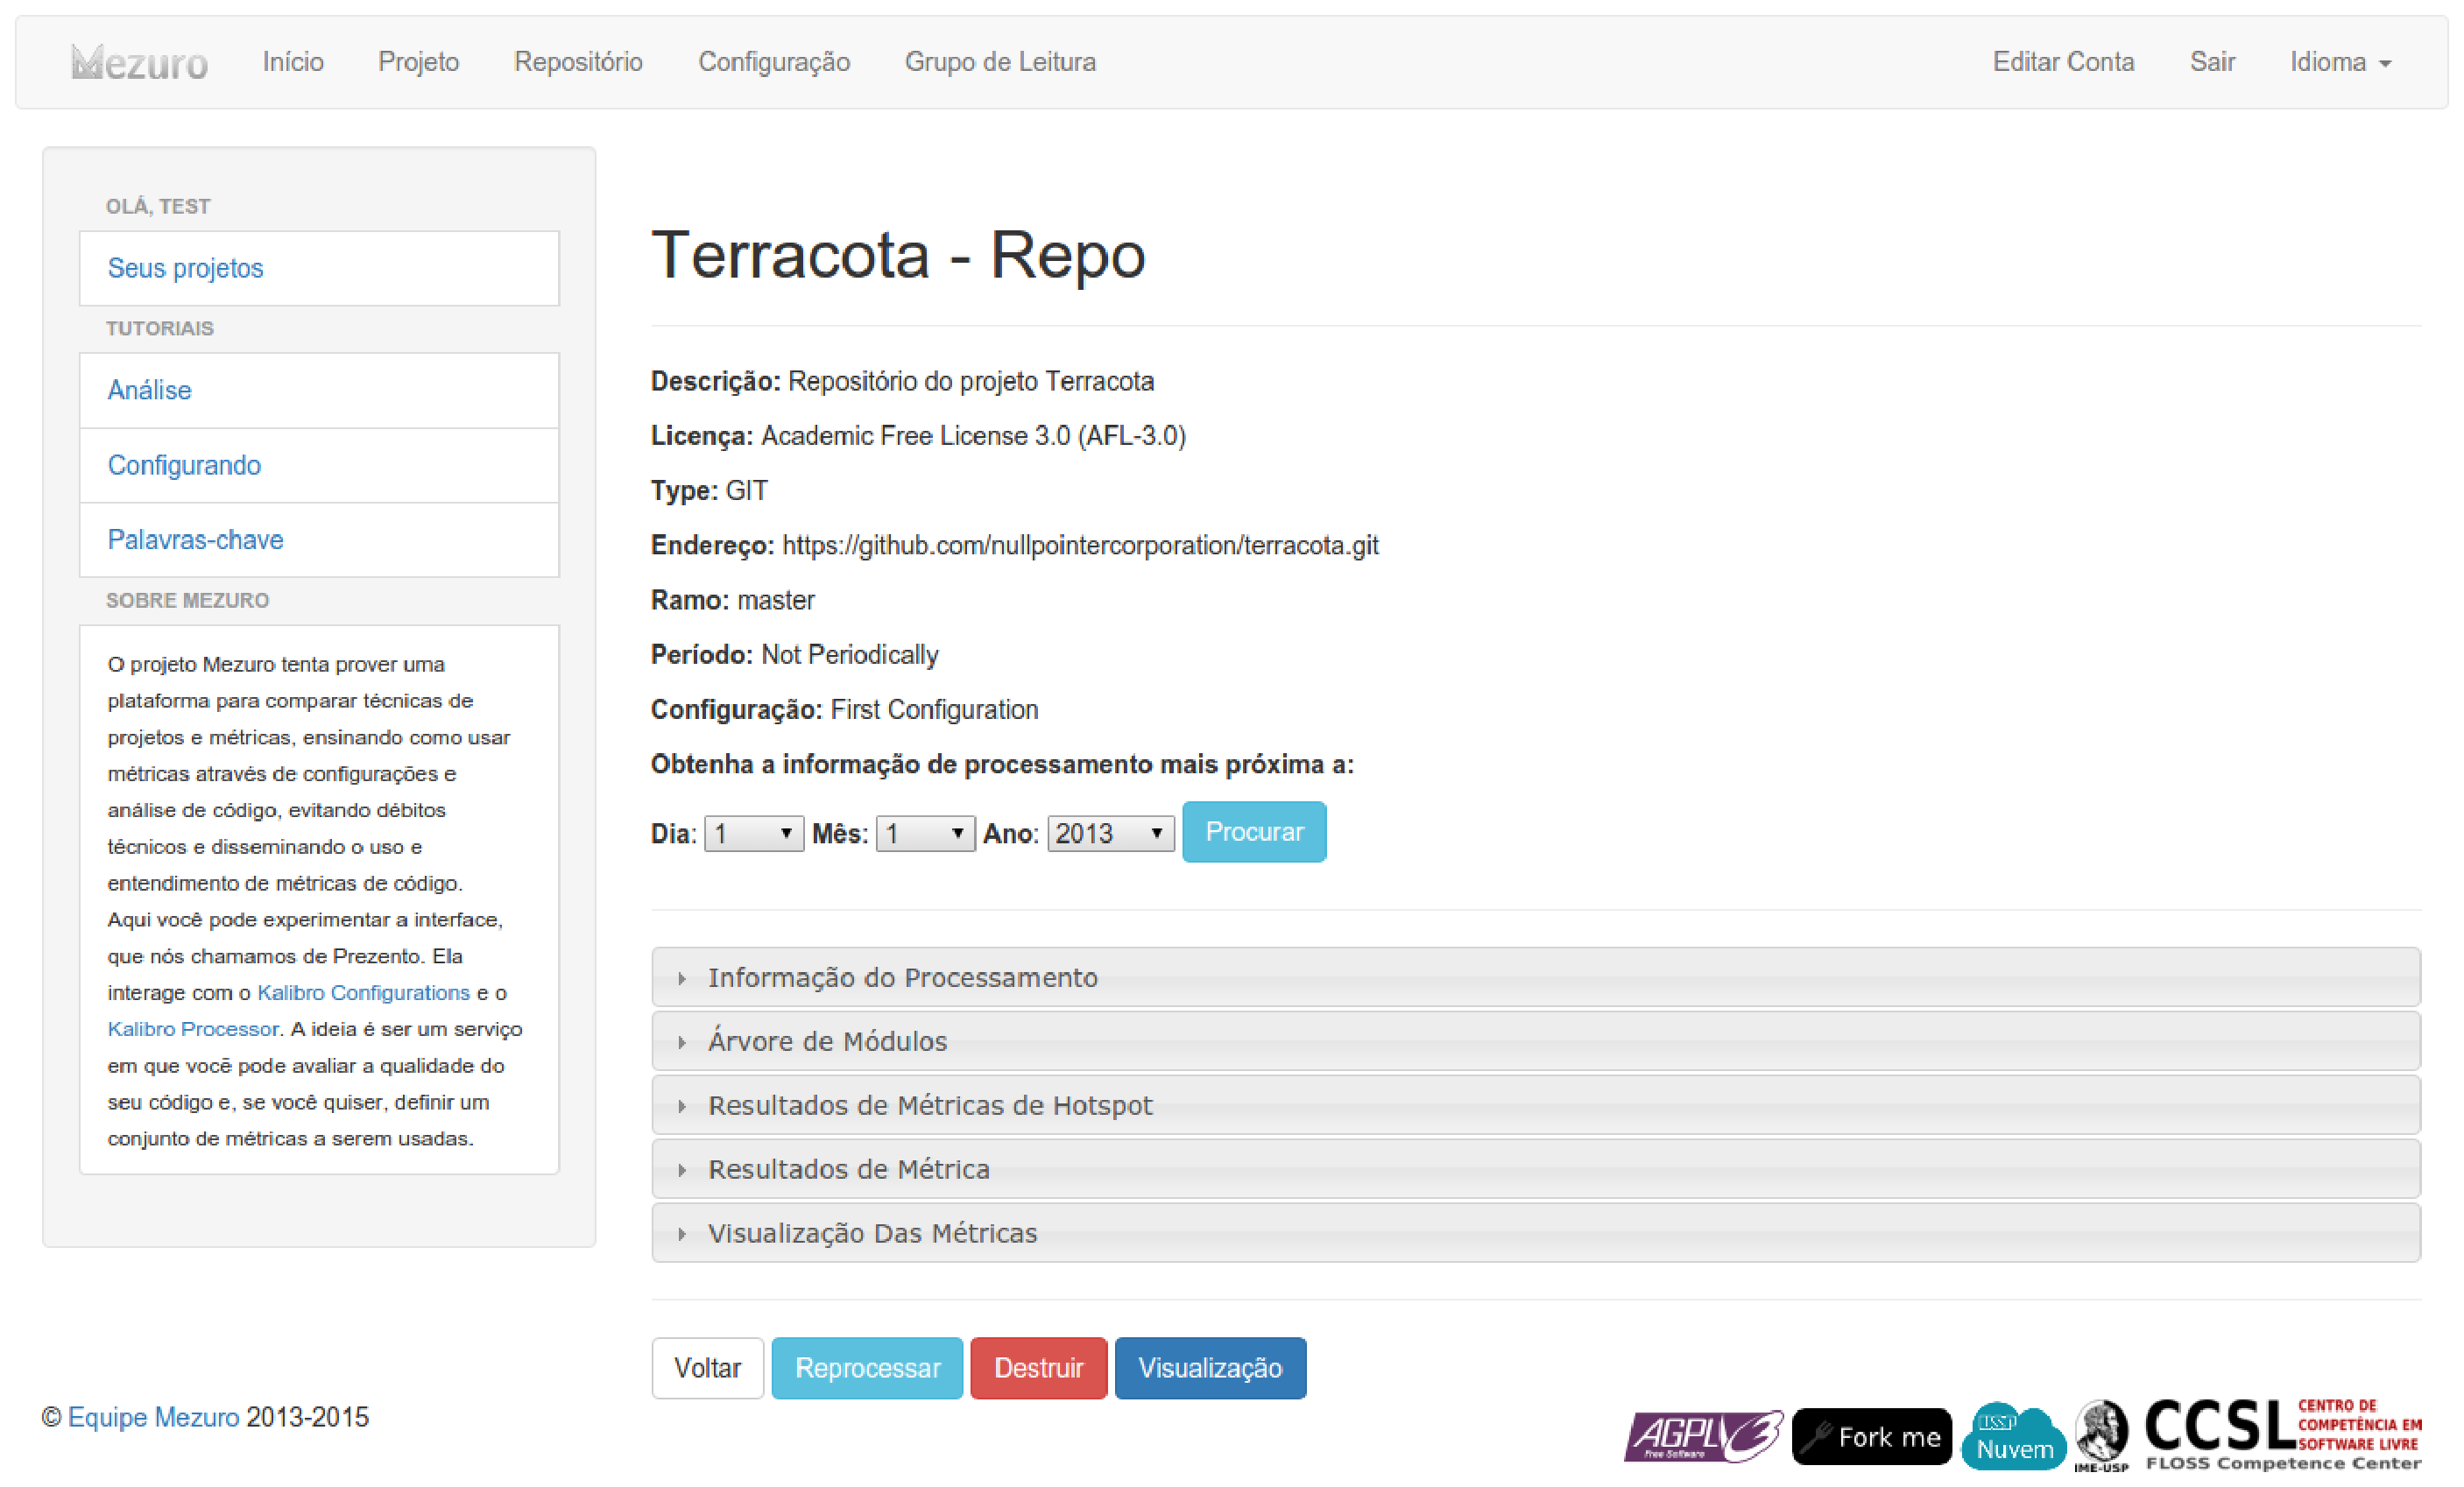
\includegraphics[keepaspectratio=true,scale=0.33]
    {figuras/exmplo_disposicao_botao_visualizacao_1.eps}
  \caption{Possíveis disposições dos botões de acesso à visualização (recolhido)}
  \label{fig:exmplo_disposicao_botao_visualizacao_1}
\end{figure}

\begin{figure}[!htb]
	\centering
    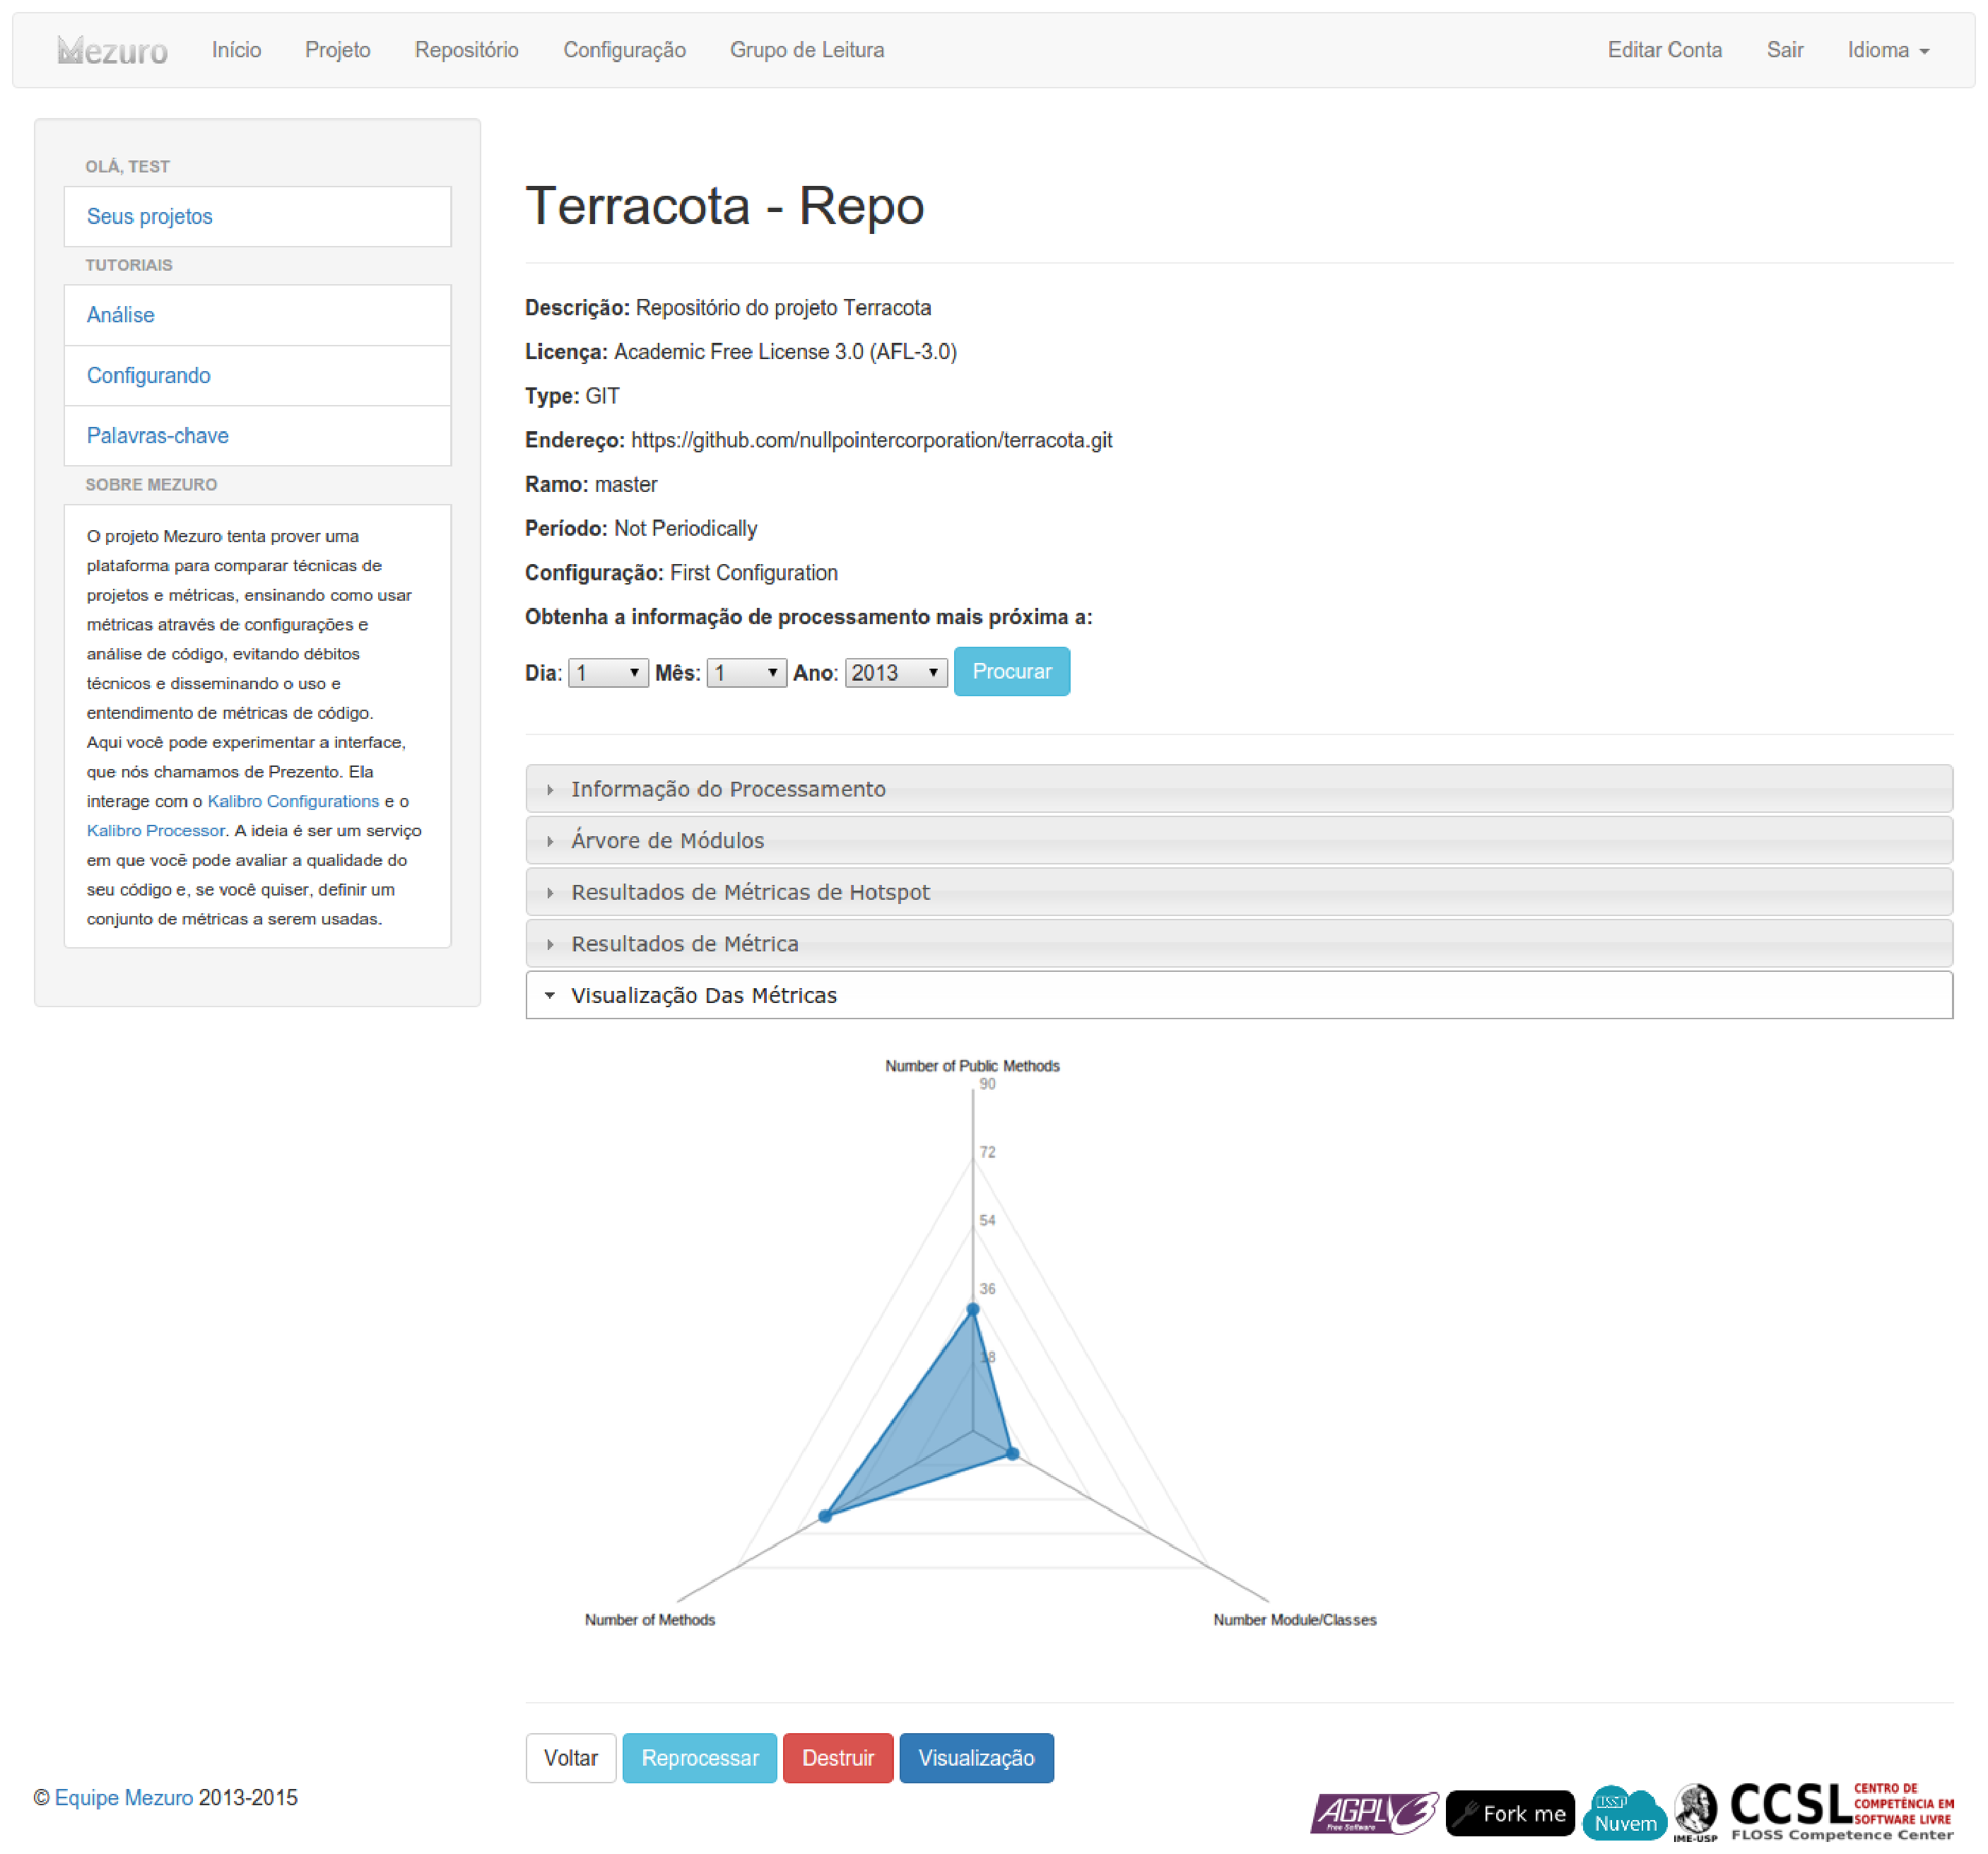
\includegraphics[keepaspectratio=true,scale=0.33]
    {figuras/exmplo_disposicao_botao_visualizacao_2.eps}
  \caption{Possíveis disposições dos botões de acesso à visualização
  (expandido) (adptado) \cite{filgueiras2014mezuro}}
  \label{fig:exmplo_disposicao_botao_visualizacao_2}
\end{figure}

\newpage

As Figuras \ref{fig:controllers_complete} e \ref{fig:models_complete} mostram os
diagramas das camadas de Controle e de Modelo do Prezento. Foram geradas com a
\textit{gem} RailRoady\footnote{\url{http://railroady.prestonlee.com/}}.

% TODO: atualizar estes diagramas

\begin{figure}[!htb]
	\centering
    \includegraphics[keepaspectratio=true,scale=0.33]
    {figuras/controllers_complete.eps}
  \caption{Diagrama da Camada de Controle}
  \label{fig:controllers_complete}
\end{figure}

% TODO: realocar posição de algumas classes na figura da camada de Modelo (+1)

\begin{figure}[!htb]
	\centering
    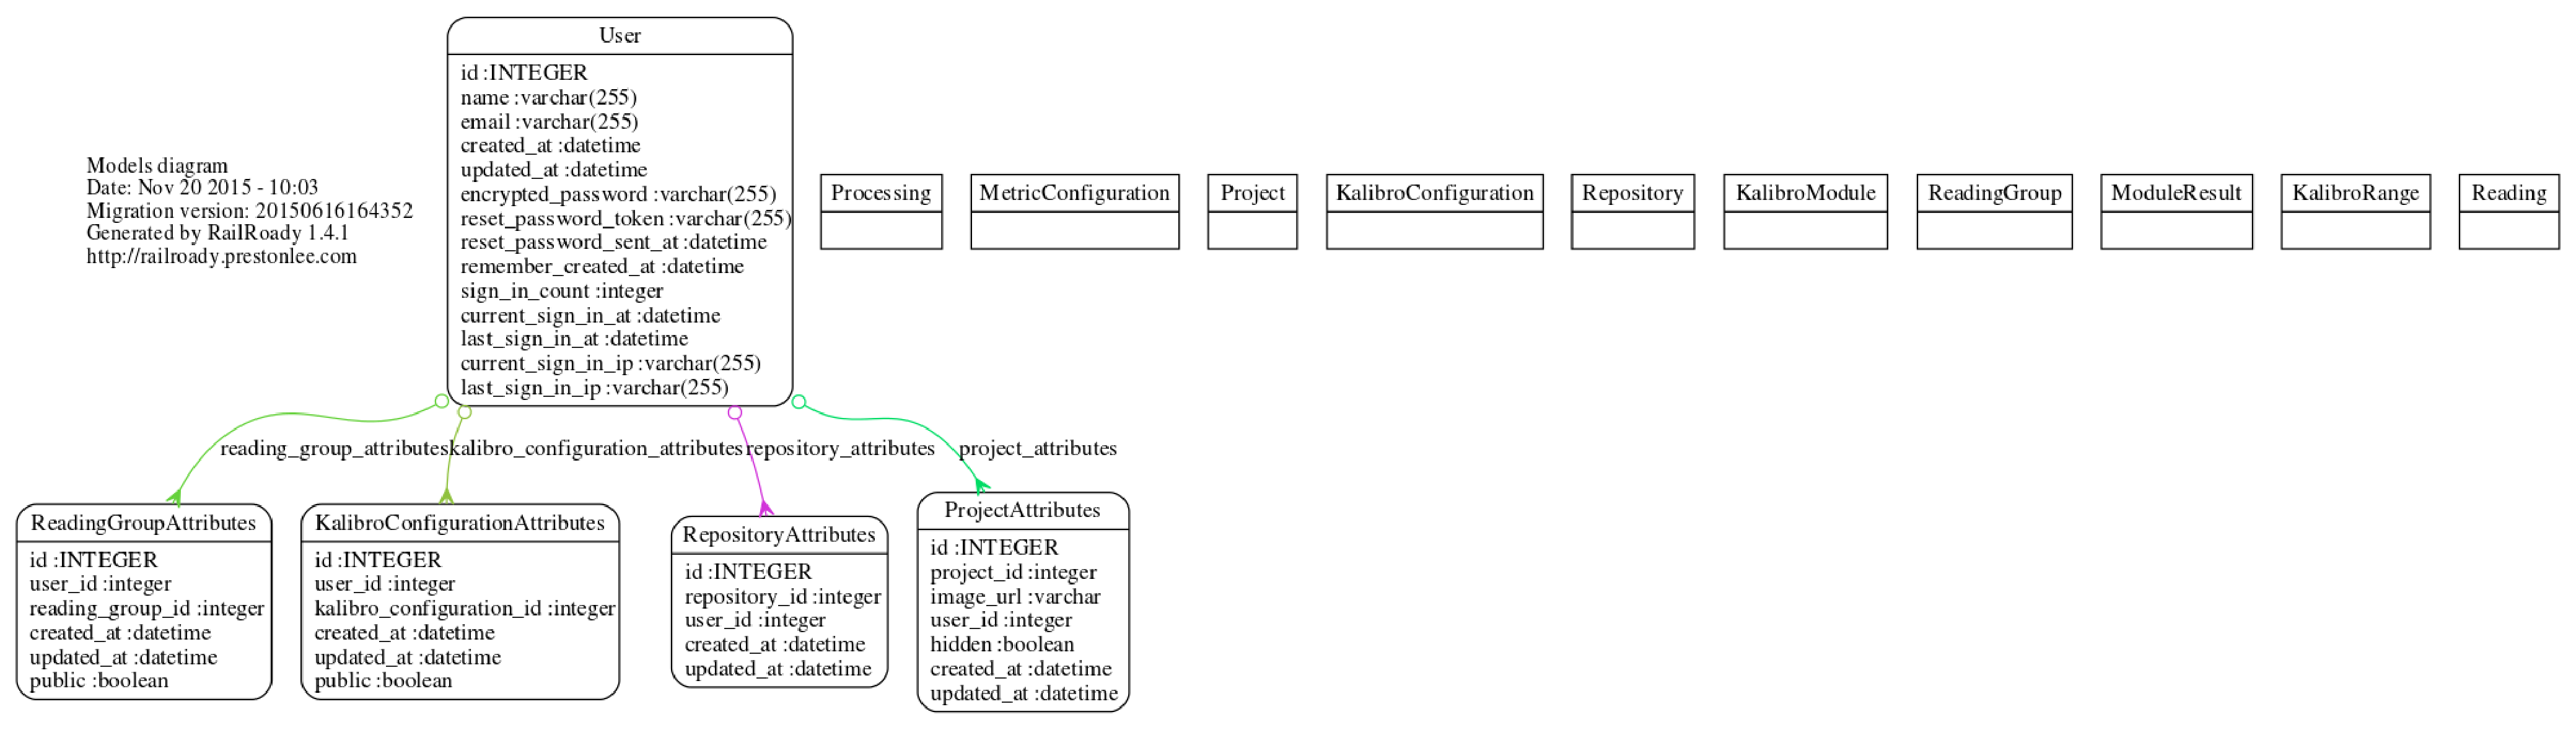
\includegraphics[keepaspectratio=true,scale=0.25]
    {figuras/models_complete.eps}
  \caption{Diagrama da Camada de Modelo}
  \label{fig:models_complete}
\end{figure}

\newpage

E a Figura \ref{fig:prezento_folders} mostra a organização dos diretórios. Os
principais pacotes envolvidos na realização deste trabalho serão:

\begin{itemize}
  \item app/assets/javascripts/: para a adição dos arquivos Javascript de
  geração das visualizações;
  \item app/views/: para adição do meio de interação do usuário com a
  visualização;
  \item spec/ ou tmp/: para a adição temporária dos arquivos extraídos dos
  resultados da análise em determinado formato que auxiliará na geração das
  visualizações.
\end{itemize}

% TODO: essa imagem é realmente necessária?

\begin{figure}[!htb]
	\centering
    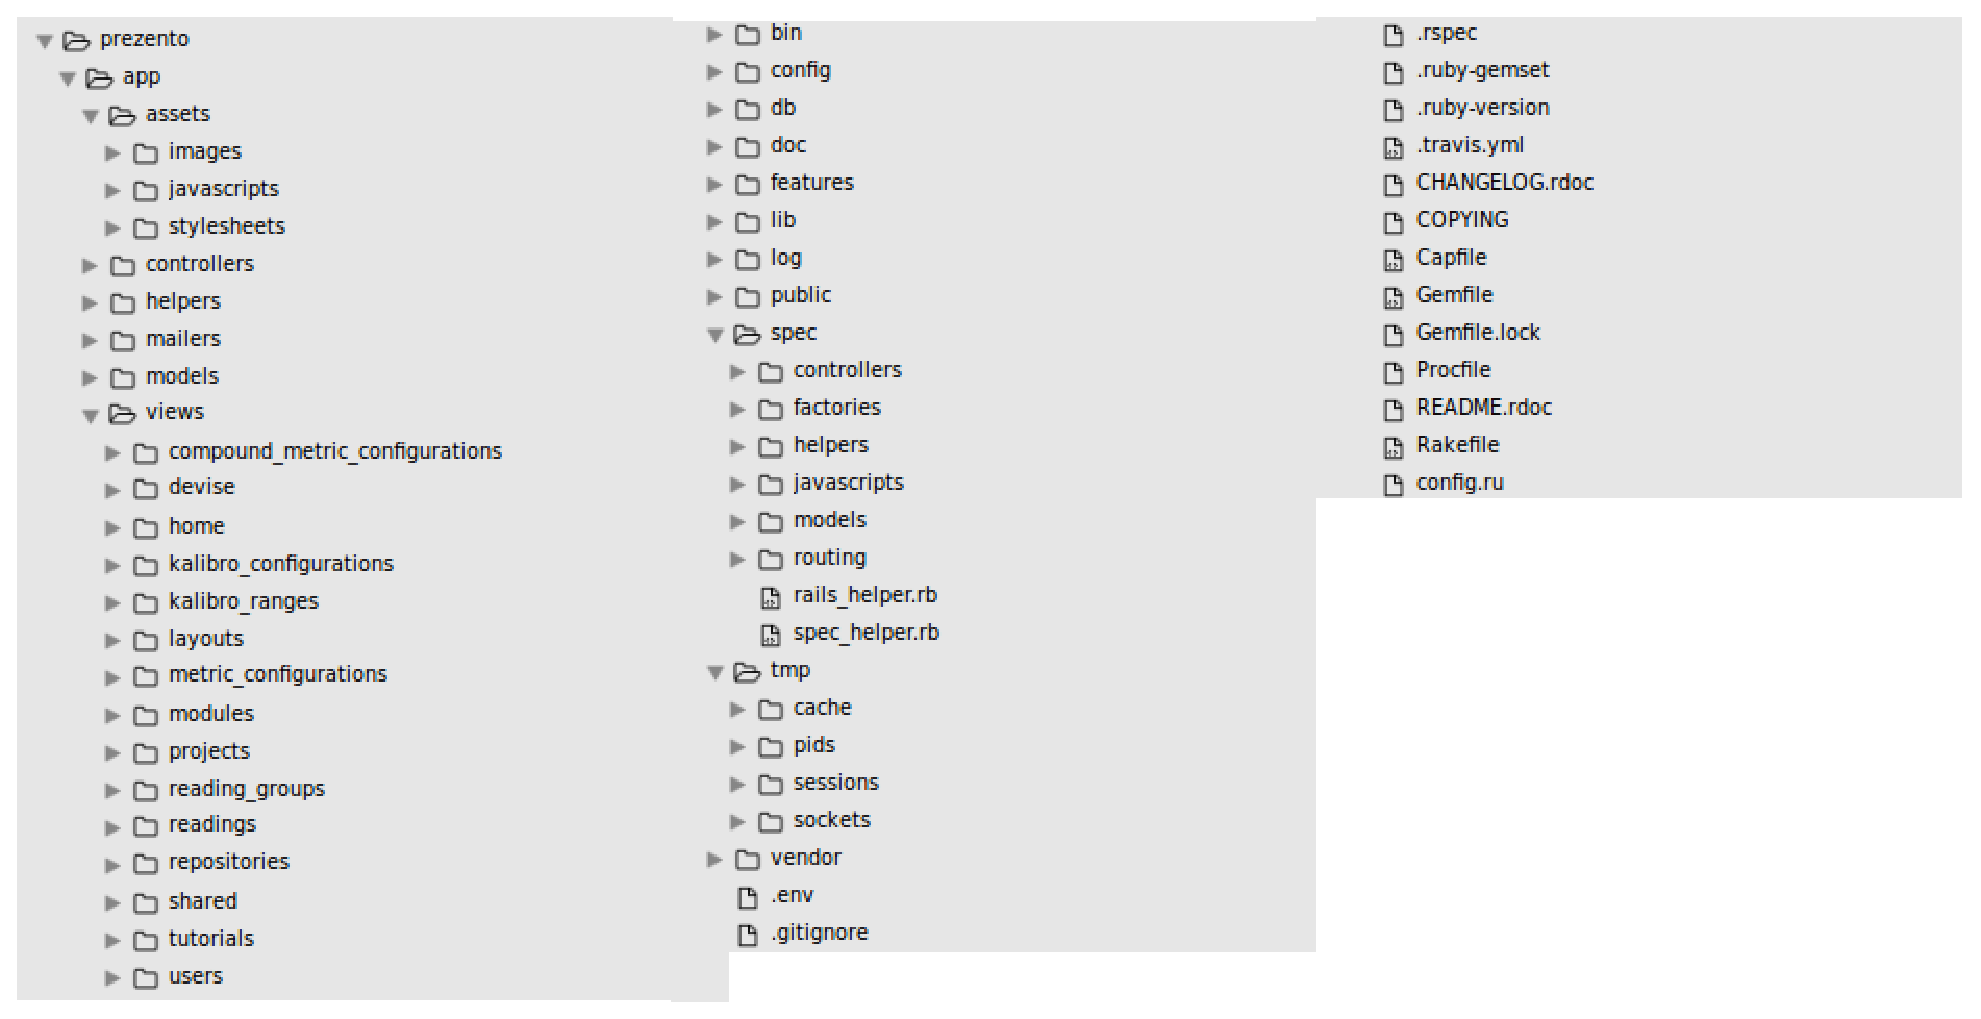
\includegraphics[keepaspectratio=true,scale=0.5]
    {figuras/prezento_folders.eps}
  \caption{Organização dos Diretórios do Prezento}
  \label{fig:prezento_folders}
\end{figure}

\newpage

\section{D3 - Data-Driven Documents}

D3.js (\textit{Data-Driven-Documents}) é uma biblioteca Javascript construída
inicialmente por \citeonline{bostock2011d3}, que tem como um dos seus objetivos
principais a produção de visualizações dinâmicas e interativas para a Web. Ela
faz uso de várias tecnologias vastamente utilizadas: HTML (para o conteúdo das
páginas), SVG (para descrição de gráficos vetoriais) e CSS (para estética das
páginas). A Figura \ref{fig:d3_gears} é um exemplo de como esse uso (ou
interação) é feito. Esta biblioteca permite ao programador manipular o Modelo de
Objeto de Documento (do inglês, \textit{Document Object Model} - DOM), para
modificar determinada seleção de elementos na página. Essa modificação, seja
adição ou remoção de elementos, depende dos dados de entrada e é onde a
aplicação de transformações dinâmicas é feita. Os autores idealizaram a união de
três preocupações: compatibilidade, depuração e desempenho \cite{bostock2011d3}.

\begin{figure}[!htb]
	\centering
    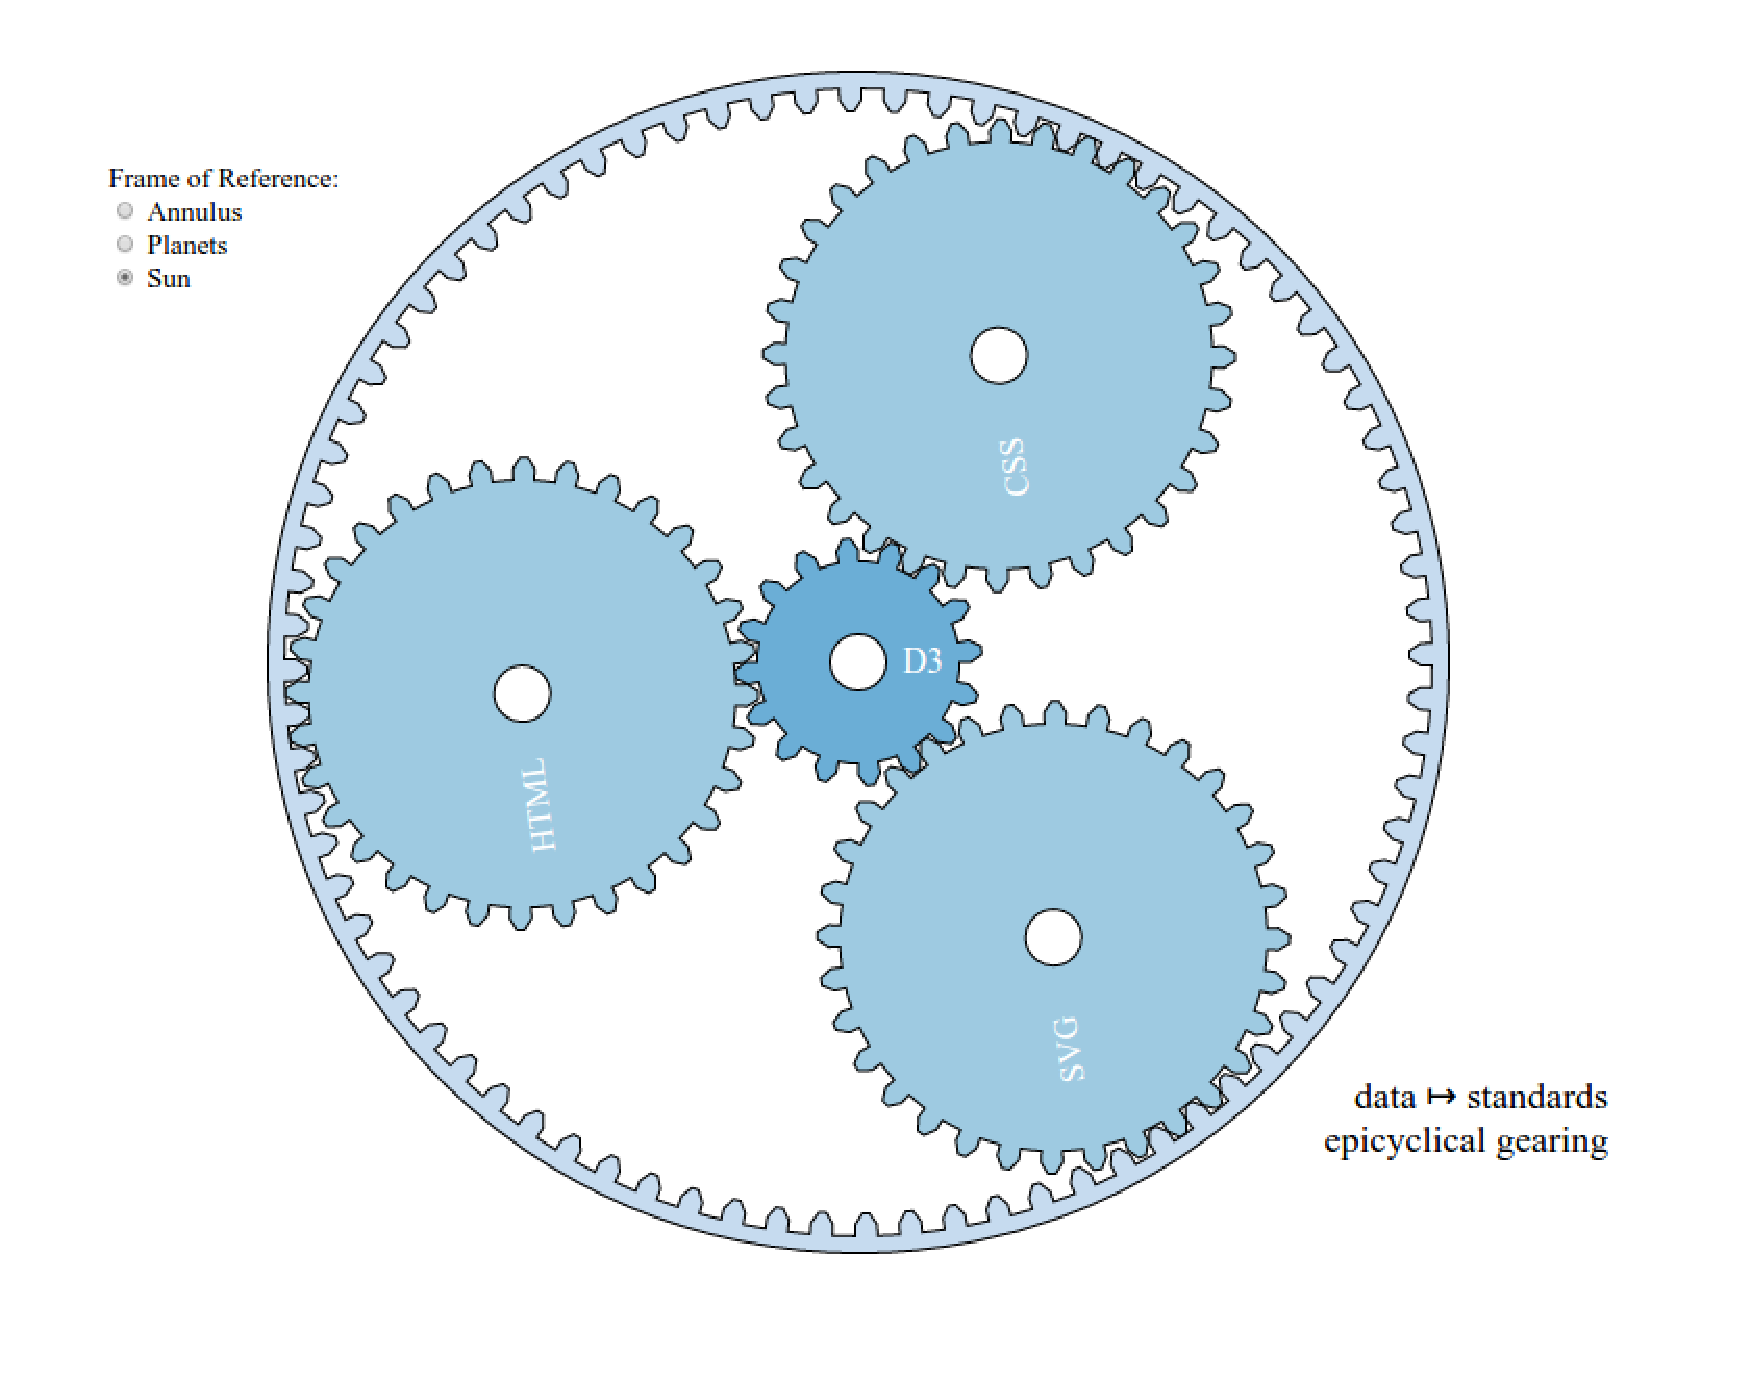
\includegraphics[keepaspectratio=true,scale=0.5]
    {figuras/d3_gears.eps}
  \caption{Exemplificação do Uso das Tecnologias pela D3.js \cite{michaeld3}}
  \label{fig:d3_gears}
\end{figure}

A biblioteca D3.js é licenciada sob a \textit{BSD licenses}, que é compatível
com a licença do Mezuro (\textit{AGPL} - \textit{Version} 3) e possui uma vasta
galeria de exemplos que podem se adaptar ao proposto neste trabalho.

\begin{figure}[!htb]
	\centering
    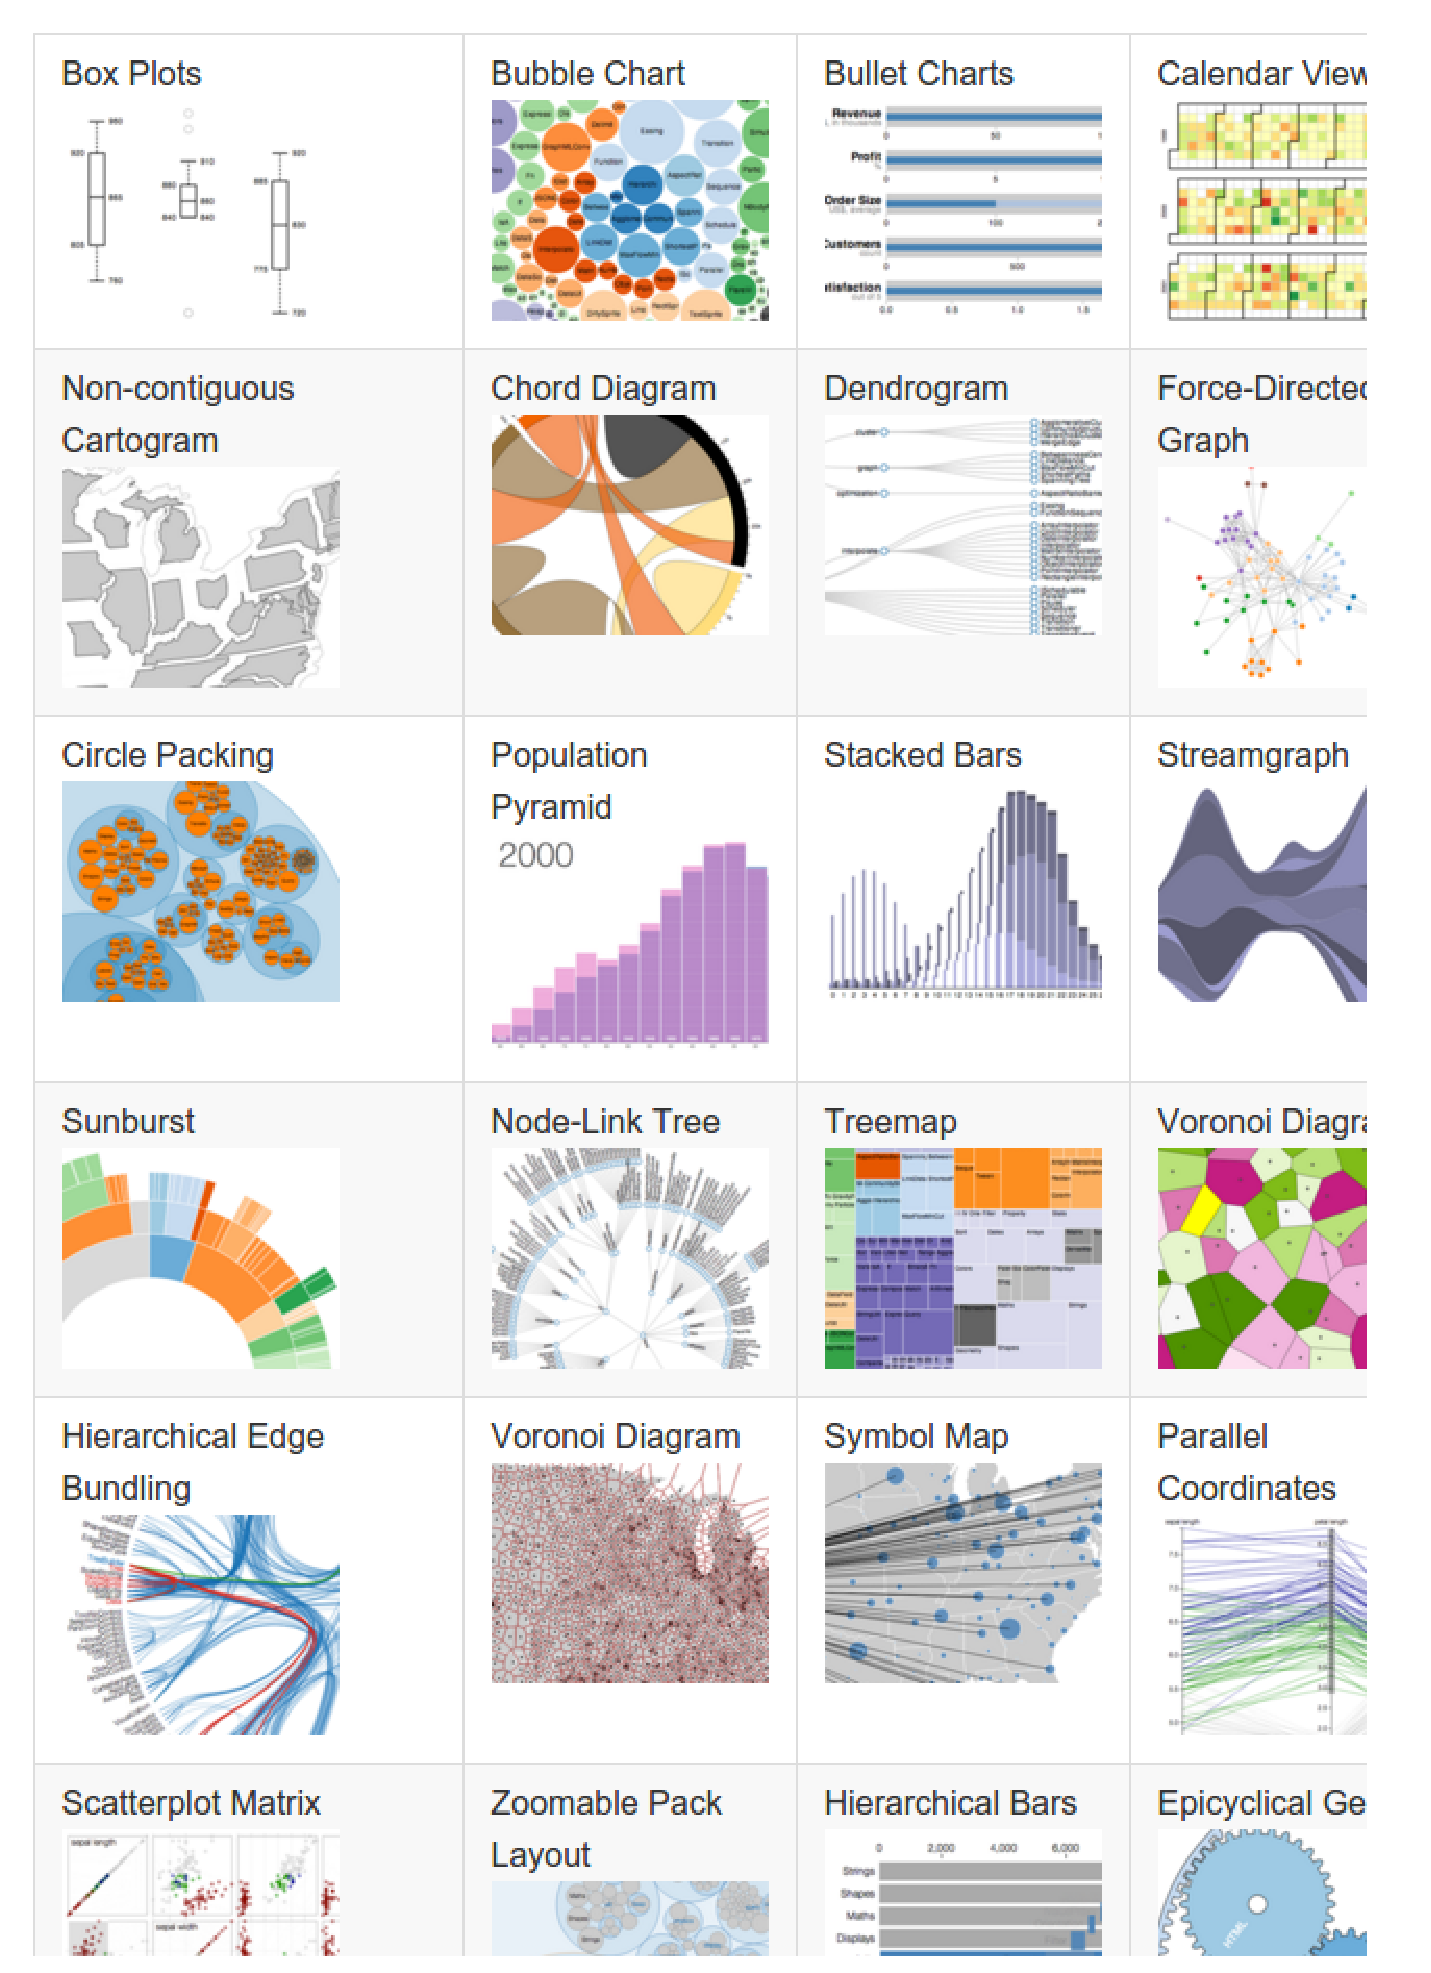
\includegraphics[keepaspectratio=true,scale=0.5]
    {figuras/d3_gallery.eps}
  \caption{Galeria de Exemplos da biblioteca D3.js \cite{galleryD3}}
  \label{fig:d3_gallery}
\end{figure}

https://github.com/mbostock/d3/wiki/Gallery

\section{Exemplo de Uso}

% TODO: escolher 3 projetos para serem alvo
% TODO: escolher quais métricas

\subsection{Resultados Econtrados}

\section{Visualização - Gráfico Radar}
